\documentclass{beamer}
\usepackage[utf8]{inputenc}

\usetheme{Madrid}
\usecolortheme{default}
\usepackage{amsmath,amssymb,amsfonts,amsthm}
\usepackage{txfonts}
\usepackage{multicol}
\usepackage{tkz-euclide}
\usepackage{listings}
\usepackage{adjustbox}
\usepackage{array}
\usepackage{tabularx}
\usepackage{gvv}
\usepackage{lmodern}
\usepackage{circuitikz}
\usepackage{tikz}
\usepackage{graphicx}
\usepackage{hyperref}

\setbeamertemplate{page number in head/foot}[totalframenumber]

\usepackage{tcolorbox}
\tcbuselibrary{minted,breakable,xparse,skins}



\definecolor{bg}{gray}{0.95}
\DeclareTCBListing{mintedbox}{O{}m!O{}}{%
  breakable=true,
  listing engine=minted,
  listing only,
  minted language=#2,
  minted style=default,
  minted options={%
    linenos,
    gobble=0,
    breaklines=true,
    breakafter=,,
    fontsize=\small,
    numbersep=8pt,
    #1},
  boxsep=0pt,
  left skip=0pt,
  right skip=0pt,
  left=25pt,
  right=0pt,
  top=3pt,
  bottom=3pt,
  arc=5pt,
  leftrule=0pt,
  rightrule=0pt,
  bottomrule=2pt,
  toprule=2pt,
  colback=bg,
  colframe=orange!70,
  enhanced,
  overlay={%
    \begin{tcbclipinterior}
    \fill[orange!20!white] (frame.south west) rectangle ([xshift=20pt]frame.north west);
    \end{tcbclipinterior}},
  #3,
}
\lstset{
    language=C,
    basicstyle=\ttfamily\small,
    keywordstyle=\color{blue},
    stringstyle=\color{orange},
    commentstyle=\color{green!60!black},
    numbers=left,
    numberstyle=\tiny\color{gray},
    breaklines=true,
    showstringspaces=false,
}
%------------------------------------------------------------
%This block of code defines the information to appear in the
%Title page
\title %optional
{4.10.2}
\date{September 16,2025}
%\subtitle{A short story}

\author % (optional)
{Aditya Appana - EE25BTECH11004}



\begin{document}


\frame{\titlepage}
\begin{frame}{Question}
The distance of the point of intersection of the lines $2x$ $-$ $3y + 5= 0$ and $3x + 4y = 0$
from the line $5x$ $-$ $2y = 0$ is \rule{1.5cm}{0.15mm}.
\end{frame}



\begin{frame}[fragile]
    \frametitle{Solution}
We need to find the point of intersection of the lines $2x$ $-$ $3y + 5= 0$ and $3x + 4y = 0$, which we can do by forming the augmented matrix. \\
\begin{align}
\myvec{2 & -3 & -5 \\ 3 & 4 & 0}
\end{align}

Using row transformations:
\begin{align}
\myvec{2 & -3 & 5 \\ 3 & 4 & 0} \xrightarrow{\text{R_2 \rightarrow $R_2- \frac{3}{2}R_1$}} \myvec{2 & -3 & 5 \\ 0 & \frac{17}{2} & \frac{-15}{2}} 
\end{align} 

Solving, we get the point of intersection as \begin{align}\myvec{\frac{-20}{17} \\ \frac{15}{17}}\end{align}
\end{frame}


\begin{frame}[fragile]
    \frametitle{Solution}
Two find the distance of this point from the line $5x$ $-$ $2y = 0$, we use the formula:
\begin{align}
\left|\frac{\vec{n}^T\vec{x} - c}{||n||}\right| = d \\
\left|\frac{\myvec{5\\-2}^T\myvec{\frac{-20}{17} \\ \frac{15}{17}}}{\sqrt{5^2 + 2^2}}\right| = 
\left|\frac{-130}{17\sqrt{29}}\right| = \frac{130}{17\sqrt{29}} = d
\end{align}

The distance of the point of intersection of the lines $2x$ $-$ $3y + 5= 0$ and $3x + 4y = 0$
from the line $5x$ $-$ $2y = 0$ is $\frac{130}{17\sqrt{29}}$.
\end{frame}

\begin{frame}[fragile]
    \frametitle{Python, C, Python+C Codes}

\href{https://github.com/AdityaAppana/ee1030-2025/tree/5566ea7440201ccd9272d7bb9e0aff34b15ff365/ee25btech11004/matgeo/4.10.2/Codes}{codes permalink}

\end{frame}

\begin{frame}
\frametitle{Plot}
\begin{figure}[H]
    \centering
    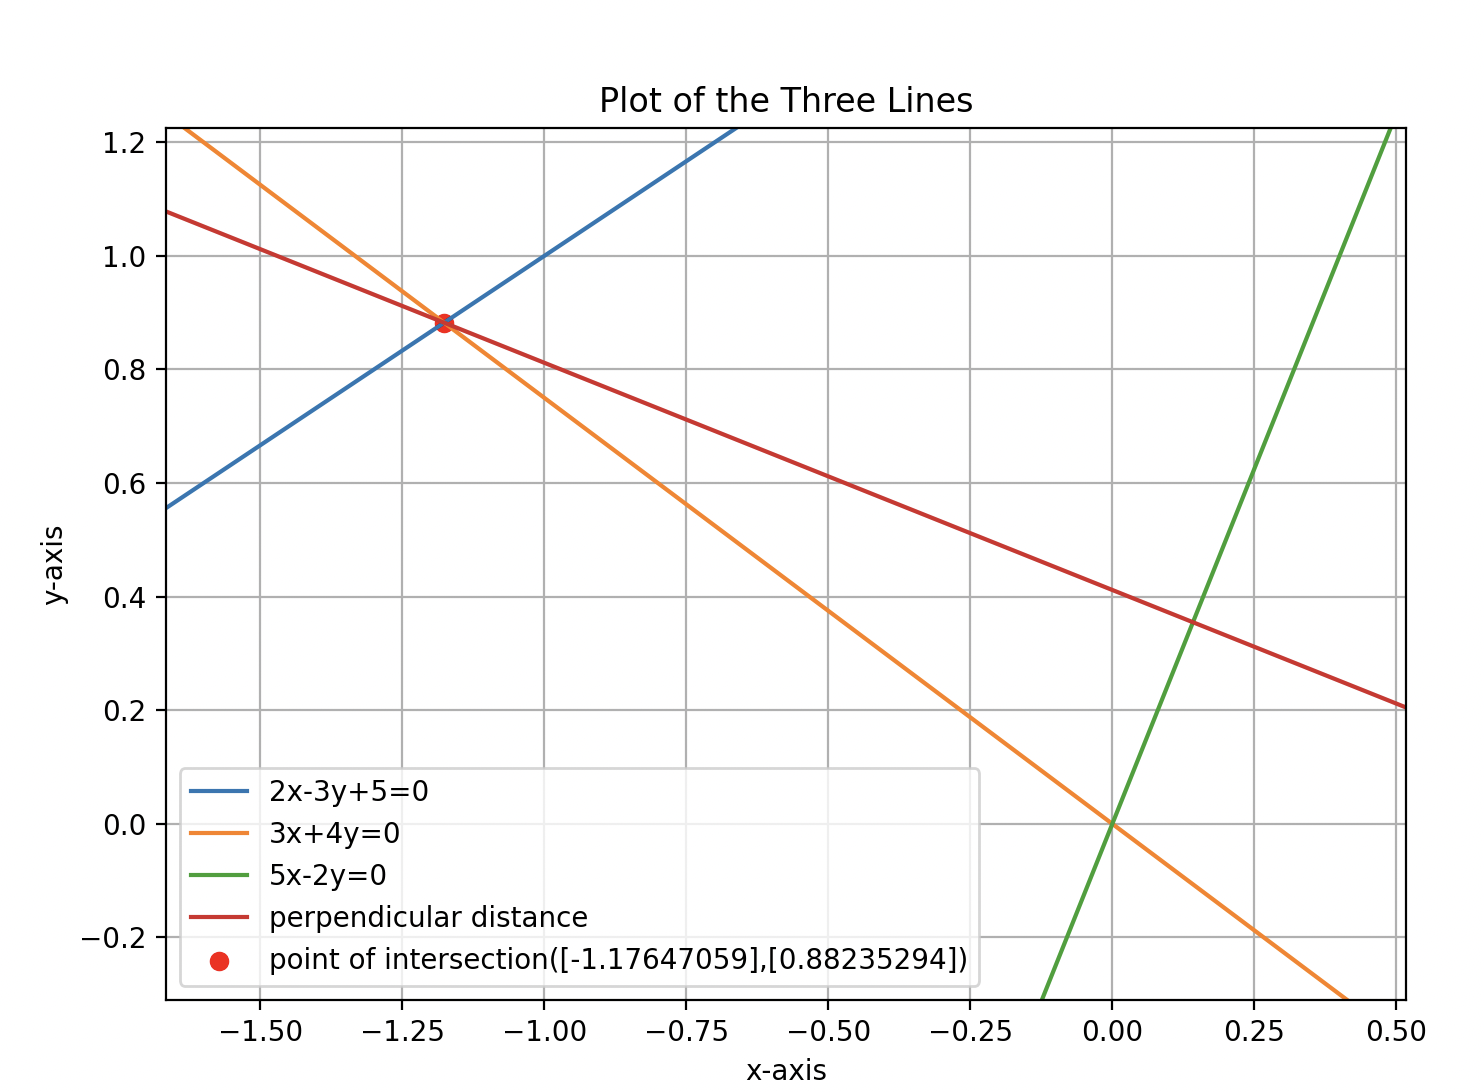
\includegraphics[width=0.6\columnwidth]{Figs/Threelines.png}
    \caption{Plot}
    \label{fig:placeholder}
\end{figure}

\end{frame}



\end{document}